\chapter{Поддержка создания предметно-ориентированных решений в системе QReal}
\label{chapter:implementation}

\section{Введение}
В данной главе описываются технологические средства для разработки предметно-ориентированных 
визуальных языков, реализованные под руководством автора в системе QReal. Описаны 
средства для разработки языков с использованием метаредактора (в соответствии с <<классической>> 
методикой): сам метаредактор, редактор конкретного синтаксиса, редактор ограничений, 
редактор правил рефакторингов, средства генерации редакторов и инструментальной поддержки. 
Также описаны реализованные средства поддержки методики <<метамоделирования на лету>>.
Приводится описание эксперимента по сравнению времени, необходимого для создания редактора
языка, генератора для него, ограничений и правил рефакторинга с использованием платформы QReal 
и наиболее распространённых из её аналогов.

\section{Возможности ядра системы QReal}
Прежде чем переходить к описанию средств описания визуальных языков, необходимо кратко 
описать возможности системы, в рамках которой будут работать созданные по метамоделям 
редакторы и средства инструментальной поддержки. \ac{dsmPlatform} QReal построена по 
модульному принципу: имеется абстрактное ядро, реализующее общую для всех языков функциональность 
и инфраструктуру редакторов, в него как подключаемые модули (плагины) загружаются редакторы, 
реализующие специфику конкретных языков, и инструменты, реализующие какую-либо ещё 
специфичную для конкретного \ac{DSM}-решения функциональность. Ядро не содержит в себе 
никаких знаний про конкретные языки и работает со всеми \ac{DSM}-решениями одинаковым образом. 
Всю необходимую информацию о языке и действиях, которые можно выполнить над диаграммами, 
созданными с его помощью, ядро получает из плагинов, либо непосредственно из метамодели 
языка, если ядро работает в режиме интерпретации метамодели. Общая архитектура системы 
представлена на рисунке~\ref{qRealArchitecture}.

\begin{figure} [ht]
	\begin{center}
		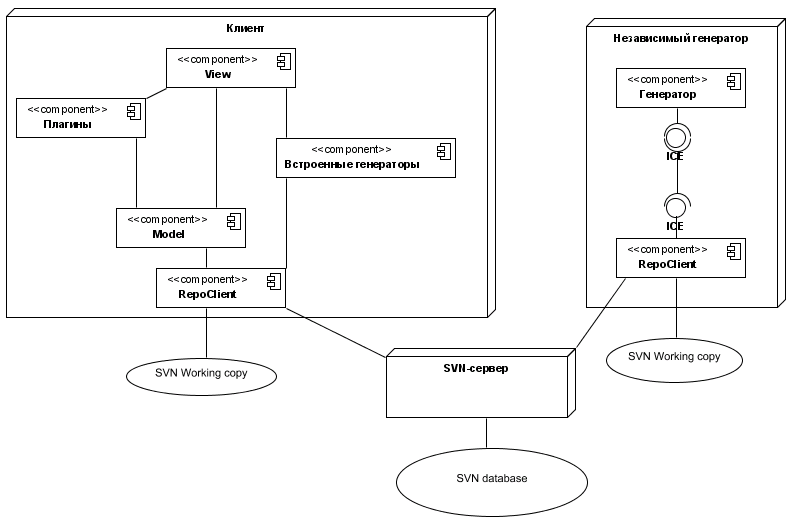
\includegraphics[width=0.7\textwidth]{part4/qRealArchitecture.png}
		\caption{Общая архитектура системы QReal.}
		\label{qRealArchitecture}
	\end{center}
\end{figure}

Плагины-инструменты могут настраивать внешний вид и состав интерфейса QReal под свои 
нужды, базовый интерфейс среды представлен на рисунке~\ref{qRealUi}. Интерфейс содержит 
область для редактирования диаграммы, называемую сценой, редактор свойств, палитру 
элементов, обозреватели логической и графической моделей, <<миникарту>>, панель инструментов и меню.

\begin{figure} [ht]
	\begin{center}
		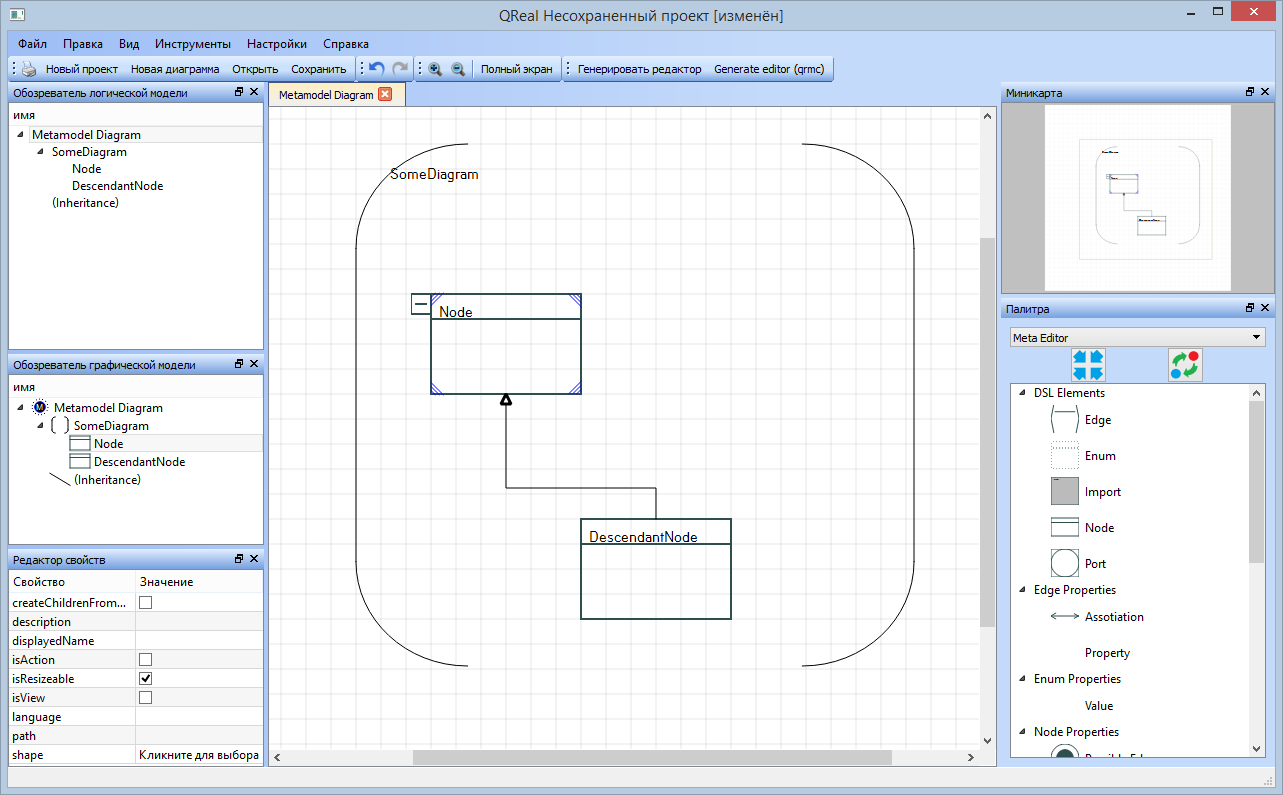
\includegraphics[width=\textwidth]{part4/qRealUi.png}
		\caption{Пользовательский интерфейс системы QReal.}
		\label{qRealUi}
	\end{center}
\end{figure}

Палитра элементов инициализируется описанными в плагине-редакторе элементами. Одновременно 
могут быть подключены несколько плагинов, тогда создаётся  несколько палитр, между 
которыми можно переключаться с помощью выпадающего списка. В палитру попадают только 
те элементы, которые имеют графическое представление, элементы, которые его не имеют, 
считаются абстрактными и используются в качестве базовых для определения других элементов.

Редактор свойств отображает все свойства выделенного в данный момент элемента и даёт 
возможность их редактировать. Свойство характеризуется своим именем (задаваемым в метамодели), 
типом (одним из фиксированного набора элементарных типов, типом-перечислением или 
типом-ссылкой на другой элемент диаграммы) и значением по умолчанию. Для разных типов 
редактор свойств предлагает разные средства редактирования, например, выпадающие списки 
для типов-перечислений, поля ввода для строк, <<галочки>> для булевых свойств.

Панель инструментов содержит элементы, общие для всех редакторов (сохранение/загрузка, 
отмена операции и т.д.), и область, в которую добавляются действия из плагинов-инструментов. 
Действие может вызвать произвольный код из плагина, который может использовать достаточно 
богатый программный интерфейс ядра QReal, предоставляющий доступ к сохранённой в репозитории 
модели, сцене, возможность подписываться на системные события (например, закрытие вкладки 
с диаграммой, изменение системных настроек).

Любой редактор визуального языка обязан реализовывать определённый интерфейс, чтобы 
быть подключенным к ядру системы. Этот интерфейс определяет информацию, которую настраиваемый 
визуальный редактор, входящий в ядро системы, должен знать о синтаксисе визуального 
языка, чтобы давать возможность создавать диаграммы. С точки зрения ядра системы подключаемый 
визуальный редактор представляет собой набор диаграмм (различных визуальных языков, 
входящих в состав редактора, их может быть несколько), каждая диаграмма содержит в 
себе список элементов. Элемент может быть либо узлом, либо связью. Любой элемент обладает 
списком свойств (свойства с точки зрения абстрактного синтаксиса представляют собой 
тройки <<имя - тип - значение по умолчанию>>) и внешним видом. Внешний вид узла задаётся в 
векторном графическом формате, близком к SVG~\cite{svg}, но с некоторыми расширениями 
(возможностью определить порты, к котором могут подключаться связи и областями для вывода значений 
свойств из репозитория). Внешний вид связи определяется стилем линии (сплошная, пунктирная 
и т.д.) и видом конца линии, выбираемым из нескольких предопределённых значений (открытая 
и закрытая стрелки, закрашенный и незакрашенный ромб и т.д.). Для узла также указывается, 
какие связи можно к нему подключить и какие узлы он может содержать внутри себя как 
составные элементы.

Редактор визуального языка можно создать вручную, реализовав описанный выше интерфейс 
на языке C++ и собрав подключаемую библиотеку. Однако такой подход весьма неэффективен, 
поэтому был использован лишь однажды, для нужд тестирования системы. Далее речь пойдёт 
об автоматизации создания визуальных редакторов. Здесь был дан лишь краткий обзор 
возможностей ядра системы, необходимый для дальнейшего изложения, более подробно 
см. статьи~\cite{terekhov2009architecture, kuzenkova2011qreal, kuzenkova2013qreal}.

\section{Инструментальные средства поддержки создания визуальных языков}

\subsection{Метаредактор}
В системе QReal для быстрого создания редакторов используется визуальный метаязык и 
соответствующий редактор, называемый метаредактором. По визуальной метамодели языка, 
созданной в метаредакторе, генерируется код на C++, реализующий интерфейс подключаемого 
модуля, который требуется ядру системы.

\subsubsection{Визуальный метаязык}
В основу метаязыка системы QReal заложены принципы, используемые, например, в метаязыке MOF~\cite{mof}: 
элементы моделируемого языка (сущности и связи) моделируются сущностями метаязыка 
(Node и Edge), эти сущности могут быть связаны отношениями наследования и <<является контейнером для>>. 
И сущность, и связь могут иметь свойства, значения для которых можно задавать при 
редактировании модели в редакторе свойств QReal. Имеется ряд вспомогательных элементов 
метаязыка, определяющих поведение элементов языка при взаимодействии с ними пользователя, 
например, позволяет ли контейнер располагать внутри себя элементы произвольным образом, 
или сам располагает элементы подряд друг под другом. Подробнее об имеющихся элементах 
см. в приложении~\ref{appendixB}.

\subsubsection{Особенности языка}
Метаязык QReal имеет следующие особенности, важные для создания CASE-инструментов 
промышленного уровня.

\begin{enumerate}
	\item Принцип <<Если функциональность не требуется, о ней можно не знать>>. Для создания
		языка требуется использовать следующие сущности: <<метамодель>>, <<диаграмма>>,
		<<узел>>, <<связь>>. Остальные элементы можно добавлять в метамодель по мере необходимости,
		генерация редактора возможна без них.
	\item Возможность определения нескольких языков в рамках одной метамодели. 
	\item Возможность задания отношения вложенности между элементами.
	\item Типизированные порты --- они дают возможность различать места на фигуре, к которым 
		могут быть подключены связи, и по-разному обрабатывать связи в зависимости от 
		того, к какому конкретно порту они подключены.
	\item Отношение раскрытия (или эксплозия) позволяет реализовать иерархическую декомпозицию
		в редакторе. При задании этого отношения можно указать, как редактору следует его 
		обрабатывать --- следует ли обязательно создавать целевой элемент при создании 
		элемента-источника, следует ли помещать целевой элемент на <<пользовательскую палитру>>.
		Нужно это для реализации подпрограмм в тех языках, где есть это понятие (например, QReal:Robots).
		Для некоторых языков раскрытие не имеет семантики подпрограммы (например, вложенные пакеты
		в UML), поэтому семантики раскрытия и настраивается в метаредакторе.
\end{enumerate}

\subsubsection{Генерация редакторов}
Созданную в метаредакторе метамодель можно использовать для того, чтобы получить редактор, 
несколькими способами: сгенерировать исходный код редактора непосредственно по метамодели, 
сгенерировать сначала XML-описание, а затем по XML-описанию исходный код редактора, 
либо открыть метамодель в интерпретаторе метамоделей и обойтись вовсе без генерации. 
Схематически разные способы представлены на рисунке~\ref{image:editorGeneration}.

\begin{figure} [ht]
	\begin{center}
		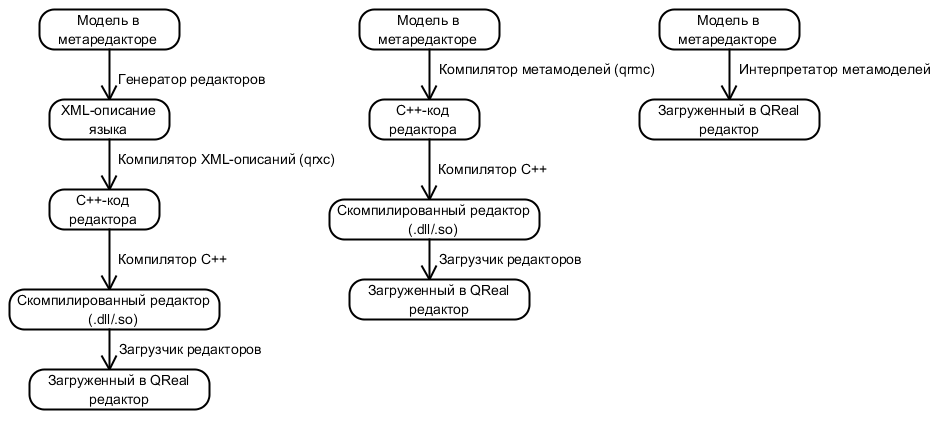
\includegraphics[width=\textwidth]{part4/editorGeneration.png}
		\caption{Получение редактора по метамодели.}
		\label{image:editorGeneration}
	\end{center}
\end{figure}

Способ, использующий XML-описание метамодели, концептуально сложнее, чем генерация кода
по метамодели напрямую, но он более устойчив к изменениям в метаязыке --- XML-описания
при необходимости легко поправить вручную, файлы с метамоделью требуют метаредактора
версии, которая может их редактировать. Поэтому большинство языков в QReal используют
сейчас схему с промежуточным XML-представлением.

Структура XML-файла практически полностью соответствует структуре метамодели языка 
(точнее, визуальный метаязык появился как визуализация существующего XML-языка). 
Синтаксис языка был впервые предложен в дипломной работе А.А. Симоновой в 2007 году, 
однако претерпел с тех пор ряд значительных изменений. Новые возможности ядра QReal 
реализуются сначала в XML-языке, а уже затем переносятся в метаязык, и на данный момент 
XML-язык обладает возможностями, которые в метаязыке пока отсутствуют. Пример такой 
возможности --- задание групп в палитре. Эта возможность позволяют собрать близкие 
по смыслу элементы языка и сворачивать или разворачивать в палитре группы элементов. 
Также есть возможность задать одновременное создание сразу нескольких элементов, например, 
чтобы при создании диаграммы поведения робота на неё сразу же добавлялся блок <<начало>>, 
обязательный для всех диаграмм.

Интерпретатор метамоделей позволяет избежать необходимости генерации кода на C++ и 
компиляции редактора. Метамодель языка, подготовленная в метаредакторе, загружается 
в интерпретатор, и он с её помощью эмулирует поведение сгенерированного плагина-редактора. 
При таком подходе скорость работы системы несколько меньше, чем в случае скомпилированного 
редактора (в работе~\cite{tarasova2015editors} приводятся результаты эксперимента по сравнению скоростей
выполнения типичных операций). Однако отсутствие необходимости пересобирать редактор после каждого изменения 
языка значительно снижает время цикла <<разработка-тестирование>> для вносимых в язык 
изменений. Кроме того, интерпретатор делает возможным внесение в метамодель изменений 
прямо в процессе работы с редактором языка, поэтому применение такого подхода необходимо 
для реализации инструментальной поддержки режима <<метамоделирования на лету>>.
На данный момент в QReal применяется и генеративный, и интерпретативный подходы к 
созданию редакторов, интерпретатор используется для быстрого прототипирования языка, 
генераторы --- для финализации языка и создания инсталляционных пакетов, поставляемых 
пользователям. 

Для того, чтобы гарантировать, что результирующие редакторы ведут себя 
одинаково для одной метамодели языка вне зависимости от способа получения редактора, 
была разработана и включена в процесс сборки тестирующая система, создающая тестовые 
редакторы для нескольких разных метамоделей всеми тремя способами и проверяющая, что 
функции интерфейса редактора во всех трёх случаях возвращают одинаковый результат.
Метамодели выбраны так, чтобы использовать все возможности ядра системы, обеспечивая 
достаточно высокий уровень тестового покрытия. В качестве входных данных система использует 
файл с метамоделью, по метамодели генерируются редакторы либо метамодель загружается в интерпретатор, 
после чего последовательно вызываются все методы интерфейса редактора на наборе тестовых данных, 
эмулирующих взаимодействие ядра QReal с редактором. Тест считается пройденным, если все методы
вернули одинаковый результат.

\subsection{Редактор формы фигур}
Редактор формы фигур предназначен для задания конкретного синтаксиса языка и представляет 
собой простой векторный редактор, запускаемый из метаредактора при редактировании свойства 
<<Форма>> узла. Использовать существующие графические редакторы оказалось невозможным 
в связи с тем, что требуется задавать не только внешний вид элемента, но и поведение 
элемента при взаимодействии с ним пользователя --- куда можно подключать связи, как 
должна изменяться форма элемента при его растягивании или сжатии, где выводить значения 
свойств из репозитория.

Редактор позволяет использовать изображения, заранее подготовленные в обычных графических 
редакторах, в качестве элементов создаваемой формы фигуры, например, так реализованы 
фигуры блоков в QReal:Robots. 

Изображения могут быть дополнены точечными и линейными портами. Порт --- место на 
фигуре, к которому можно подключить связь, точечный порт отличается от линейного тем, 
что к линейному порту связь может подсоединяться в любом месте линии. Порт может иметь 
тип, один из заранее определённых в метамодели, для связи может быть указано, к портам 
какого типа её разрешено подключать.

Имеется возможность задать отображение статического текста и динамического текста. 
Динамический текст --- поле на фигуре, текст для которого берётся из свойства фигуры в 
репозитории. В редакторе формы фигур указывается имя свойства, откуда надо брать значение. 
В процессе рисования диаграммы на созданном языке подставляется 
реальное текущее значение свойства, кроме того, значение свойства можно редактировать 
прямо на сцене. Статический текст --- это нередактируемая надпись на элементе, указываемая
при задании формы элемента. 

Для каждого элемента изображения можно определить условие, при котором он будет отображаться. 
Условие задаётся в виде логического выражения, в котором можно использовать значения 
свойств элемента. 

Результат создания формы фигуры может быть сохранён в виде XML-строки как свойство 
элемента Node в метамодели либо как отдельный XML-файл, который можно переиспользовать 
при создании других фигур.

\subsection{Редактор ограничений}
Ограничения необходимы для того, чтобы, во-первых, минимизировать вероятность ошибок 
при разработке системы, во-вторых, чтобы иметь возможность обнаружить ошибку как можно 
раньше. Наличие средств задания ограничений позволяет существенно повысить удобство 
пользования визуальной технологией и повысить качество программ, создаваемых с её помощью, 
поэтому средства задания ограничений очень распространены в существующих \ac{DSM}-платформах. 

Ограничения бывают двух видов --- ограничения на состояние разработанной системы во 
время её работы и ограничения на модель системы в процессе её разработки. Первый 
вид ограничений схож с операторами assert в текстовых языках программирования, второй --- 
с синтаксическими проверками кода, выполняемыми компилятором или средой разработки. 
В случае \ac{DSM}-платформы первый вид ограничений может быть реализован только для частных 
случаев, в рамках разрабатываемых с помощью \ac{DSM}-платформы визуальных технологий. Второй 
же вид ограничений может описываться на уровне метамодели визуального языка, в этом 
случае ограничения могут автоматически проверяться редактором диаграмм. Далее речь 
пойдёт исключительно про второй вид ограничений.

Задание ограничений на создаваемую модель частично происходит в самой метамодели, 
правила синтаксиса языка не позволят создать некорректную диаграмму, если редактор строго 
им следует (что в случае \ac{DSM}-платформ практически всегда так, потому что редактор 
определяется метамоделью). Насколько сложные ограничения можно задать в метамодели 
языка зависит от используемого метаязыка. Например, метамодель UML использует для задания 
ограничений полноценный текстовый язык OCL, позволяющий писать сколь угодно сложные запросы 
к репозиторию с моделью и накладывать сколь угодно сложные ограничения на её состояние.

В системе QReal в соответствии с принципом <<не надо знать то, чем не пользуешься>> 
сложные ограничения задаются отдельно от метамодели, с помощью модели ограничений. 
Метамодель может быть создана без ограничений, они могут быть добавлены в язык потом,
по мере осознания разработчиками языка их необходимости, и отдельно, без внесения 
изменений в метамодель. Кроме того, в соответствии с идеологией предметно-ориентированного 
визуального моделирования ограничения задаются с помощью специально созданного для 
этого предметно-ориентированного визуального языка. Данный язык, а также средства 
проверки ограничений, разработанные под руководством автора данной работы, 
описаны в статье~\cite{deripaska2013constraints}, ниже приводится лишь краткое описание данных средств.

Модель ограничений создаётся после создания метамодели языка (или совместно с ней), 
также имеется возможность задавать ограничения, проверяемые для всех метамоделей (например, 
что связи должны быть обязательно подсоединены к узлам). Модель ограничений состоит 
из набора ограничений на узлы и связи. Для каждого узла или связи возможно указать 
ограничения на значение его свойств, для узла можно указать ограничения на входящие 
и исходящие связи, на содержащиеся в узле элементы или наоборот, на содержащий узел 
элемент, для связи --- на узлы, с которых начинается или которыми заканчивается связь. 
Для каждого ограничения можно указать его важность --- предупреждение или критическая 
ошибка. В случае нарушения ограничения-предупреждения элемент-нарушитель подсвечивается 
на диаграмме, в случае нарушения критического ограничения в дополнение к подсветке в 
окне ошибок появляется текстовое сообщение. 

Пример простого ограничения, применимого ко всем типам связей всех метамоделей, приведён 
на рисунке~\ref{image:constraintExample}. Ограничение требует, чтобы у любой связи существовал и начальный, и конечный 
узел (зелёный квадрат означает узел, из которого исходит связь, красный --- узел, в 
который связь входит, true означает, что они должны существовать). Ограничение имеет 
важность <<предупреждение>>.

\begin{figure} [ht]
	\begin{center}
		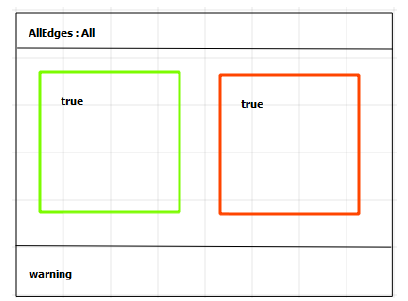
\includegraphics[width=0.5\textwidth]{part4/constraintExample.png}
		\caption{Ограничение, проверяющее наличие начального и конечного узла у связи.}
		\label{image:constraintExample}
	\end{center}
\end{figure}

Пример диаграммы с нарушением этого ограничения приведён на рисунке~\ref{image:constraintViolationExample}. 
Связь, не имеющая конечного узла, выделена средством проверки ограничений красным.

\begin{figure} [ht]
	\begin{center}
		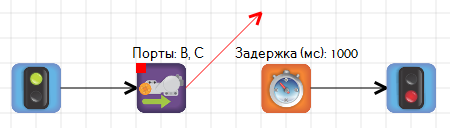
\includegraphics[width=0.7\textwidth]{part4/constraintViolationExample.png}
		\caption{Пример отображения нарушения ограничения.}
		\label{image:constraintViolationExample}
	\end{center}
\end{figure}

Механизм проверки ограничений реализован следующим образом. По модели ограничений 
генерируется код подключаемого модуля проверки ограничений на C++, который компилируется 
в динамическую библиотеку. При запуске QReal все модули проверки ограничений загружаются 
в подсистему проверки ограничений ядра QReal. При выполнении пользователем определённых 
действий (таких как изменение имени элемента, изменение значения свойства элемента, 
создание или удаление элемента, подключение или отключение связи) вызывается обработчик 
в подсистеме проверки ограничений. Обработчик быстро проверяет наличие ограничения 
на тип изменённого элемента в списке подключённых модулей проверки, а также для всех 
связей и содержащих элемент элементов, и наоборот, элементов, содержащихся в данном. 
В случае, если в подключённых модулях хоть одно такое ограничение есть, для каждого 
ограничения вызывается его проверка, результаты собираются в список и, если есть невыполненные 
ограничения, информация об этом предоставляется пользователю в виде подсветки элементов 
на диаграмме и, возможно, в текстовом виде в окне ошибок. Таким образом, несмотря на то, 
что проверка ограничений вызывается при практически любом редактировании модели, за 
счёт фильтрации ограничений по типу проверяемого объекта это не приводит к существенной 
потере производительности.

\subsection{Редактор правил рефакторинга}
Возможность автоматически применять рефакторинги для диаграмм довольно редка среди CASE-систем и \ac{DSM}-платформ, 
но стала вполне обычной для текстовых сред программирования, поэтому ожидается и от создаваемых визуальных сред, чтобы успешно конкурировать с текстовыми. 
Рефакторинг определяется как изменение внутренней структуры программы без изменения 
её видимого поведения с целью сделать её проще для понимания и упростить её сопровождение~\cite{fowler2003refactoring}. 
В случае с визуальными моделями рефакторинг может рассматриваться как изменение логической 
модели системы или как изменение внешнего вида диаграммы, не затрагивающее логическую 
модель (например, перерасположение элементов). Второй вид рефакторинга исследован 
достаточно хорошо (см. GraphViz~\cite{graphViz}, KIELER~\cite{kieler} и т.д.), система 
QReal использует компоненту GraphViz для автоматической раскладки элементов на диаграммах. 
Первый вид рефакторингов изучен гораздо меньше.

В общем случае схема рефакторинга визуальной модели такова~\cite{mens2007challenges}.
Система состоит из нескольких визуальных моделей, характеризующих систему с разных точек зрения, по моделям автоматически 
генерируется часть кода, другая часть кода, возможно, пишется вручную. При рефакторинге 
необходимо, во-первых, внести необходимые изменения в редактируемую модель, во-вторых, 
синхронизировать изменения с другими моделями, в-третьих, выполнить перегенерацию кода 
по моделям, затронутым изменениями, в-четвёртых, согласовать рукописный код. Рефакторинг 
вручную может оказаться весьма трудоёмким процессом, поэтому естественно желание его 
автоматизировать. Но для каждого визуального языка набор рефакторингов может быть свой, 
зависящий от семантики конкретного языка. Поэтому требуется задавать правила рефакторингов 
на уровне метамодели. В QReal для задания рефакторингов принят тот же подход, что и 
для задания ограничений --- правила рефакторингов, если они требуются, определяются 
в отдельной модели после определения метамодели языка, для этого используется специализированный 
визуальный язык. Ниже приводится краткое описание реализации системы рефакторингов в QReal, 
подробнее о реализации см. в статьях~\cite{kuzenkova2013refactoring, kuzenkova2012refactorings}. 
Общая схема разработки и применения правил рефакторинга представлена на рисунке~\ref{image:refactoring}.

\begin{figure} [ht]
	\begin{center}
		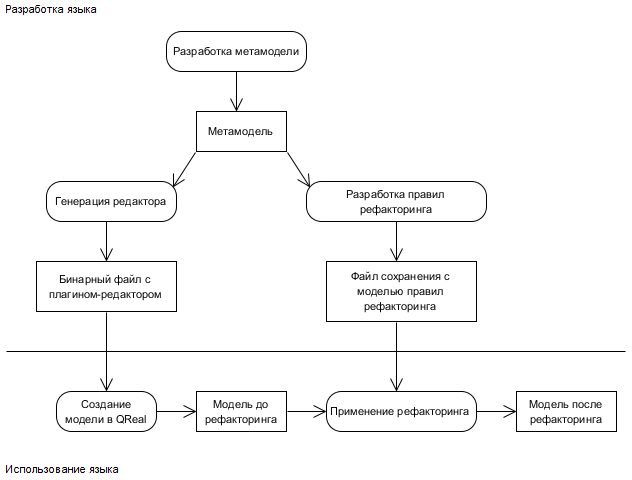
\includegraphics[width=\textwidth]{part4/refactoring.png}
		\caption{Схема разработки и применения правил рефакторинга.}
		\label{image:refactoring}
	\end{center}
\end{figure}

Язык описания правил рефакторинга имеет интересную особенность --- его элементами 
являются элементы языка, для которого определяется правило рефакторинга. Эти элементы 
автоматически подгружаются из метамодели разрабатываемого языка редактором правил 
рефакторинга и используются для определения шаблонов, которые будет сопоставлять в 
диаграмме средство выполнения рефакторинга при его применении. Сами правила задаются 
в виде графовых грамматик: правило делится на часть BEFORE, в которой задаётся шаблон, 
который ищется в диаграмме, и на часть AFTER, на которую замещается сопоставленный 
шаблон. При этом в правиле можно использовать специальные элементы, такие как <<Выделенный 
фрагмент диаграммы>>, каждому элементу можно указать его идентификатор. Элементы, 
имеющие одинаковый идентификатор в левой и правой части правила, считаются одним элементом 
и будут сохранены (возможно, с изменениями) при рефакторинге. Элементы, идентификатор 
которых не встречается в части BEFORE, будут созданы, элементы, идентификатор которых 
не встречается в части AFTER --- удалены. Можно модифицировать существующее значение 
свойства элемента, для доступа к нему используется ключевое слово EXIST. 

С технической точки зрения средство применения рефакторингов использует тот же механизм 
работы с графовыми грамматиками, что и используемый для задания семантики интерпретации 
визуальных языков. Этот механизм, а также существующие его аналоги, подробно описан в статьях%
~\cite{polyakov2013interpreters, polyakov2013semantics, polyakov2012semantics, polyakov2012interpreter}.
Физически средство применения рефакторингов реализовано как подключаемый модуль к 
QReal, поскольку, в отличие от подсистемы проверки ограничений, не требует тесной 
интеграции с ядром системы.

\subsection{Средства поддержки технологии <<метамоделирования на лету>>}
Технология <<метамоделирования на лету>> позволяет разрабатывать предметно-ориентированные 
языки, не используя метаредактор, прямо в процессе рисования диаграммы на разрабатываемом 
языке. Методологические аспекты технологии, включая описание процесса создания языка 
в соответствии с ней, описаны в разделе~\ref{chapter:metamodelingOnFly} настоящей 
работы, здесь будет кратко описана реализация инструментальных средств поддержки этой 
технологии в системе QReal. Более подробное описание реализации можно найти в статье~\cite{ptakhina2013metamodeling}.

\subsubsection{Средства разработки редактора}
Метамоделирование на лету --- это особый режим работы QReal, не доступный при работе 
с такими технологиями, как QReal:Robots. Таким образом, пользователи предметно-ориентированных 
решений, созданных на основе QReal, имеют возможность даже не знать о существовании 
такой функциональности.

При создании новой интерпретируемой метамодели будет открыто окно редактора с пустой палитрой. 
Элементы добавляются в язык через контекстное меню палитры. Если создаваемый элемент --- сущность, его
можно пометить как корневой элемент диаграммы, в этом случае он будет создаваться 
автоматически при создании диаграммы, и только он может быть в корне иерархии включения 
элементов (то есть это тот элемент, в который как в сыновья добавляются все остальные). 
Вновь созданный элемент будет иметь форму по умолчанию (прямоугольник для сущностей и обычную линию для связей) и не будет 
иметь свойств. Элемент уже можно начать использовать, например, если это корневой 
элемент нового языка, создать новую диаграмму, куда можно добавлять этот же или другие элементы. Форму 
элемента можно поменять через контекстное меню элемента. Схематически данный процесс 
показан на рисунке~\ref{image:metamodelingOnFlyCreationOfElement}.

\begin{figure} [ht]
	\begin{center}
		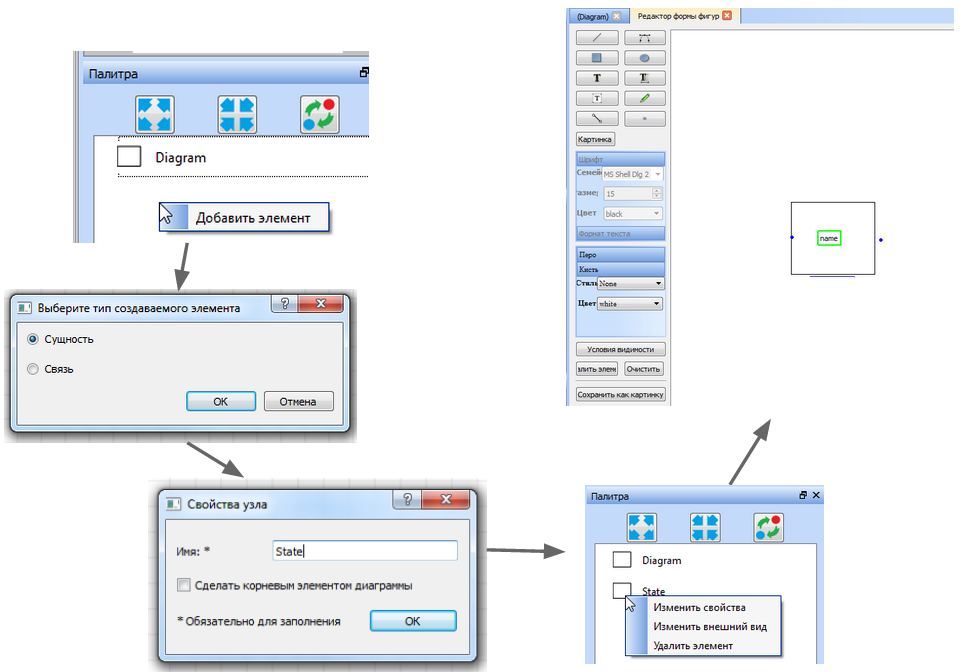
\includegraphics[width=\textwidth]{part4/metamodelingOnFlyCreationOfElement.png}
		\caption{Создание нового элемента языка.}
		\label{image:metamodelingOnFlyCreationOfElement}
	\end{center}
\end{figure}

Свойства элемента также можно добавить, удалить или отредактировать через контекстное 
меню. Свойства характеризуются своим именем, типом и значением по умолчанию. При создании нового свойства эти характеристики 
надо будет ввести, для существующих свойств их можно редактировать. При этом есть 
некоторые ограничения, связанные с поддержанием консистентности модели. Например, 
элементам, экземпляры которых уже существуют на диаграмме, нельзя добавить новое свойство 
--- уже существующие экземпляры добавленного свойства иметь не будут, что может привести 
к ошибкам в инструментальных средствах, которые рассчитаны на то, что все обозначенные 
в метамодели свойства у экземпляров элементов есть. В таком случае система запрещает 
добавление свойства и требует, чтобы до добавления свойства все экземпляры были удалены. 
При этом удаление свойства элемента безопасно --- существующие экземпляры будут иметь 
удалённое свойство, но оно никогда не будет запрошено, поскольку отсутствует в метамодели. 
Процесс редактирования свойства элемента схематически представлен на рисунке~\ref{image:metamodelingOnFlyPropertiesEditing}.

\begin{figure} [ht]
	\begin{center}
		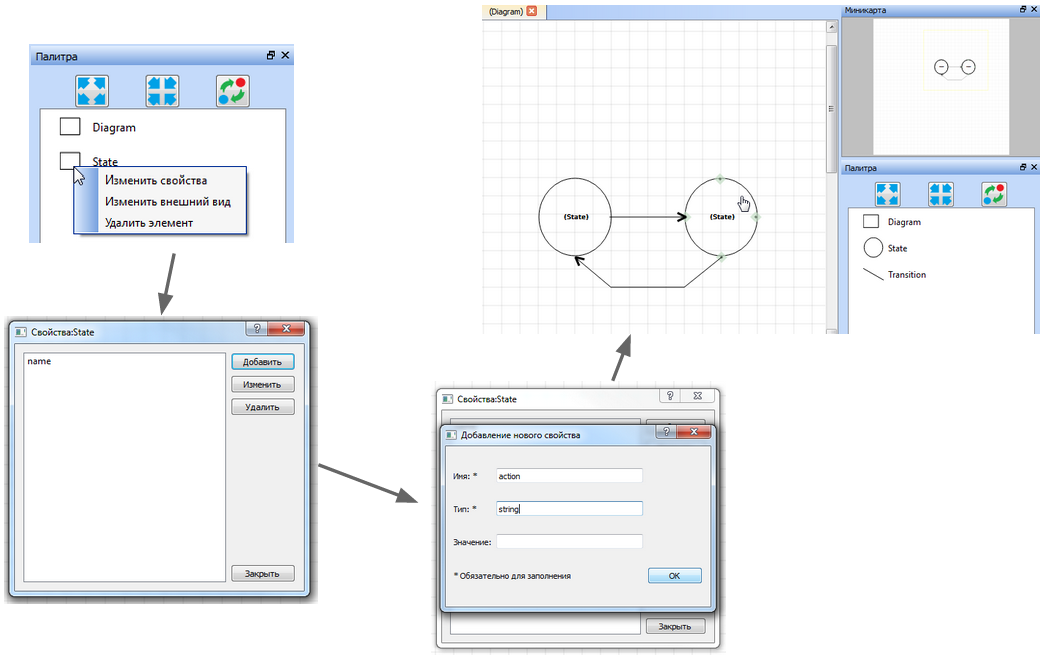
\includegraphics[width=\textwidth]{part4/metamodelingOnFlyPropertiesEditing.png}
		\caption{Редактирование свойств элемента.}
		\label{image:metamodelingOnFlyPropertiesEditing}
	\end{center}
\end{figure}

\subsubsection{Средства разработки генератора}
Средства <<метамоделирования на лету>> позволяют создавать прототип генератора для
разрабатываемого визуального языка, что делает возможным в короткие сроки создать 
прототип полноценного предметно-ориентированного решения, позволяющего создать диаграмму
и сгенерировать по ней код. Реализация средств генерации для режима <<метамоделирования на лету>>
подробно описана в статье~\cite{tikhonova2015generation}.

Для задания правил генерации используются шаблоны на текстовом языке, размеченные 
управляющими конструкциями и выражениями, позволяющими подставить в генерируемый код
значения свойств из модели. Правило генерации может быть описано для каждого элемента,
при запуске генератора вызовется правило генерации для корневого элемента модели, которое,
в свою очередь, может вызвать правила генерации остальных элементов. Правила могут быть
добавлены в процессе редактирования диаграммы с помощью контекстного меню элемента
в палитре. При этом откроется окно редактора правила, с палитрой языковых конструкций,
снабжённых контекстной справкой, и палитрой свойств элемента, для которого редактируется правило.
Редактор правил имеет синтаксическую подсветку.

Правило состоит из строк, генерируемых в целевой файл напрямую (они пишутся в кавычках) 
и ключевых слов, управляющих генерацией, таких как:
\begin{description}
	\item[foreach] позволяет обходить элементы коллекций, например, список исходящих связей;
	\item[this] позволяет обратиться к текущему генерируемому элементу модели;
	\item[if] позволяет исполнить одну из двух веток правила в зависимости от условия;
	\item[callGeneratorFor] позволяет вызвать другое правило генерации;
	\item[generateToFile] позволяет переключить выходной файл генерации.
\end{description}

Правило генерации интерпретируемо, то есть хранится как атрибут типа элемента в метамодели
и может быть вызвано сразу после своего создания. 

\section{Сравнение эффективности разработанных средств с существующими инструментами}
С целью количественного измерения эффективности разработанных в ходе диссертационного
исследования методик и инструментальных средств был проведён эксперимент по сравнению
процесса разработки визуальных предметно-ориентированных языков с помощью различных 
\ac{DSM}-платформ, включая платформу QReal. В ходе эксперимента был выбран достаточно простой визуальный
язык --- диаграммы <<сущность-связь>> в нотации Чена~\cite{chen1976er}, для которых
с использованием двух самых популярных на данный момент \ac{DSM}-платформ и платформы QReal 
был разработан редактор визуального языка, генератор в \ac{SQL} \ac{DDL}, определено 
одно семантическое ограничение (сущность должна иметь хотя бы один атрибут) и одно правило
рефакторинга (преобразование атрибута в сущность). Измерялось время реализации каждого элемента
функциональности из вышеперечисленных.

\subsection{Организация эксперимента}
Целью эксперимента было количественно проверить соответствие достигнутых в данной работе результатов
цели работы --- снижает ли предложенная методика трудозатраты при разработке инструментальных
средств для визуальных предметно-ориентированных языков по сравнению с существующими аналогами.
Было решено выполнить сравнение с двумя наиболее зрелыми и известными на данный момент 
DSM-платформами. По результатам обзора из главы \ref{chapter2} для этого были выбраны платформы
MetaEdit+\cite{kelly2008domain} и Eclipse Modeling Project~\cite{emp}. В силу ограниченности
ресурсов на проведение эксперимента было принято решение реализовать инструментальные
средства только для одного, причём достаточно простого языка. Несмотря на это, поскольку 
предлагаемые в данной работе методики ориентированы на небольшие языки, результаты можно 
считать показательными. 

Рассматривались только рекомендованные авторами технологий способы решения задачи, 
при этом не требующие кодирования на текстовых языках общего назначения. Две из трёх
участвовавших в эксперименте платформ (QReal и Eclipse Modeling Project) имеют открытые 
исходные коды, третья (MetaEdit+) предоставляет \ac{API} на основе веб-сервисов для доступа
к модели в репозитории, поэтому теоретически все эти платформы позволяют реализовать любую
функциональность. Однако в ходе эксперимента считалось, что если для реализации функциональности
требуется программирование на языке общего назначения с использованием механизмов расширения системы, 
то система не позволяет эту функциональность реализовать, в таком случае измерения не проводились.

В эксперименте участвовало два человека, имеющих опыт профессионального программирования,
разработки и использования визуальных предметно-ориентированных языков. Перед проведением
эксперимента участники создали по одному визуальному языку на всех платформах, выбранных
для измерений, чтобы ознакомиться с их возможностями. Работа над задачей эксперимента
велась совместно. Таким образом, в эксперименте моделировалась небольшая команда разработчиков, 
имеющая небольшой опыт использования выбранной \ac{DSM}-платформы,перед которой поставлена 
задача разработать полноценное \ac{DSM}-решение.

Задача, которую требовалось решить в ходе эксперимента, ставилась следующим образом.
\begin{itemize}
	\item Разработать редактор диаграмм <<сущность-связь>> в подмножестве нотации Чена со
		следующими элементами:
		\begin{itemize}
			\item Сущность (имеющая имя);
			\item Атрибут (имеет имя и тип);
			\item Отношение (имеет имя);
			\item Связь между сущностью и атрибутом;
			\item Связь между сущностью и отношением.
		\end{itemize}
	\item Разработать генератор в язык \ac{SQL} \ac{DDL}, выдающий схему базы данных по 
		диаграмме, созданной в разработанном редакторе.
	\item Реализовать проверку семантического ограничения на диаграмму --- каждая сущность
		должна быть связана хотя бы с одним атрибутом. При невыполнении этого ограничения должно 
		выдаваться предупреждение.
	\item Реализовать рефакторинг --- преобразование атрибута в сущность. При этом имя атрибута 
		должно стать именем сущности, связь с сущностью-хозяином должна быть удалена.
\end{itemize}

В ходе реализации задачи замерялось время выполнения каждого из её пунктов, включающее
в себя работу непосредственно в редакторах, поиск необходимой информации в документации, если это было необходимо, 
и борьбу с возникавшими техническими проблемами. Выбор конкретной технологии решения задачи 
и ознакомление с ней в замеряемое время не входили.

В эксперименте использовалась среда MetaEdit+ Workbench 5.1 (evaluation version)
\footnote{URL: http://www.metacase.com/download/ (дата обращения: 20.01.2016г).}
и среда Obeo Designer 8.1 Community Edition~\footnote{URL: http://www.obeodesigner.com/download (дата обращения: 20.01.2016г).}.
Из набора технологий, входящих в состав Eclipse Modeling Project, для решения задачи были выбраны
следующие.
\begin{itemize}
	\item Eclipse EMF --- для описания метамодели разрабатываемого языка и базового редактора
		логической модели, позволяющего редактировать её древовидное представление.
	\item Eclipse Sirius --- для создания визуального редактора диаграмм, соответствующего
		метамодели, и ограничений на модели, проверяемых в процессе редактирования диаграмм.
	\item Acceleo --- для создания генератора кода на текстовом языке по модели.
	\item Epsilon (точнее, Epsilon Wizard Language) --- для описания и применения правил рефакторингов.
\end{itemize}

При этом технологии Eclipse EMF, Eclipse Sirius и Acceleo входят в поставку Obeo Designer 8.1
и готовы к работе после установки этого продукта, Epsilon оказалось необходимо устанавливать
отдельно. Obeo Designer 8.1 встроенных средств поддержки рефакторингов не имеет.
Перечисленные технологии были выбраны на основании анализа времени последнего обновления
и наличия обучающих материалов среди подключаемых модулей Eclipse, предназначенных для решения
перечисленных задач.

Среда QReal в ходе эксперимента использовалась в двух режимах --- режиме визуального метаредактора
и в режиме <<метамоделирования на лету>>, учёт времени вёлся отдельно по двум режимам.

\subsection{Результаты эксперимента}
Результаты эксперимента приведены в таблице~\ref{tab:experiment}. Выполнить все требования,
перечисленные в условии эксперимента, удалось лишь в Eclipse Modeling Project и в
среде QReal в режиме метаредактора. Платформа MetaEdit+ не обладает возможностями по созданию
рефакторингов (за исключением прямой модификации модели через \ac{API} системы,
что в рамках эксперимента не рассматривалось), а средства задания ограничений оказались
недостаточно выразительными --- платформа позволяет задать ограничения вида <<не больше
заданного количества связей>>, но не позволяет задать ограничения <<не меньше>>.
Средства метамоделирования на лету системы QReal предназначены для прототипирования
языка и предполагают разработку дополнительной функциональности на последующих фазах,
после загрузки получившейся при прототипировании метамодели в метаредактор. 

\begin{table}[ht]
	\begin{longtabu} {| X[1 l p] | X[1 l p] | X[1 l p] | X[1 l p] |X[1 l p] |}
		\caption{Результаты эксперимента по созданию визуального языка} \\
		\tabucline-
		 Название DSM-платформы           & Редактор  & Генератор  & Ограничения  & Рефакторинги  \\
		\tabucline-
		\everyrow{\tabucline-}
		MetaEdit+                         & 20 минут  & 30 минут   & ---          & ---           \\
		Eclipse Modeling Project          & 2 часа    & 50 минут   & 17 минут     & 40 минут      \\
		QReal (метаредактор)              & 15 минут  & 15 минут   & 10 минут     & 15 минут      \\
		QReal (метамоделирование на лету) & 5 минут   & 15 минут   & ---          & ---
		\label{tab:experiment}
	\end{longtabu}
\end{table}

Платформа Eclipse Modeling Project показала очень большое по сравнению с остальными
платформами время создания редактора. Это связано с используемыми там гибкими, но
сложными механизмами задания редактора. Подсистема Sirius требует отдельного
описания метамодели языка, отдельного описания модели редактора, связи её с метамоделью языка
и отдельного описания палитры инструментов. При этом для описания поведения элементов палитры
используется небольшой текстово-графический язык программирования, позволяющий задавать действия
в виде дерева элементарных действий, таких как создание элемента, установки его атрибутов
и т.д. При этом возникала необходимость часто обращаться к документации, поскольку
при описании действий используется текстовый предметно-ориентированный язык, синтаксис
которого необходимо знать для создания палитры, а также много графических элементов,
семантика которых не всегда была ясна из подсказок внутри среды. Возникали и технические проблемы,
связанные с нестабильностью работы среды Eclipse. Высокие времена создания остальных
инструментов на платформе Eclipse связаны с необходимостью работы сразу в двух запущенных
экземплярах платформы, а также рутинными действиями, такими как перегенерация редактора
при изменениях в метамодели и обновление после этого всех созданных инструментов.

\subsection{Обсуждение и выводы}
\subsubsection{Обсуждение валидности}
Основная угроза валидности эксперимента связана с недостаточным количеством данных.
К сожалению, эту угрозу оказалось невозможно устранить --- полноценные эксперименты 
в области программной инженерии требуют большого количества ресурсов. Полностью валидный
эксперимент требовал бы привлечения нескольких групп разработчиков, решающих на разных
\ac{DSM}-платформах задачи, приближенные к реальным, что интересно само по себе (особенно с 
учётом отсутствия подобных опубликованных исследований), но явно выходит за рамки данного
исследования.

Важной угрозой также является предвзятость участников эксперимента --- оба участника
являются соавторами технологии QReal. Устранение этой угрозы оказалось невозможно
опять-таки в силу ограниченности времени и ресурсов. Участники эксперимента старались
проводить его настолько непредвзято, насколько возможно. Следует отметить при этом, что
и в случае реализации задачи на системе QReal требовалось обращаться к документации.

Следующая угроза --- выбор языка и корректность результатов эксперимента для других языков.
Язык диаграмм <<сущность-связь>> относится к графовым статическим языкам по введённой 
в главе~\ref{chapter1} классификации, к этому классу относится довольно много практически полезных 
предметно-ориентированных языков. Размер языка намеренно взят небольшим, поскольку
исследуемые методы предназначены для небольших проектов, к тому же это позволило закончить
задачу эксперимента за разумное время. Существенно повысить валидность позволила бы реализация
ещё одного языка, из другого класса (например, редактора для сетей Петри, с поддержкой
операционной семантики), это представляется важной частью методики проведения более масштабного
эксперимента, что является важным направлением дальнейшей работы.

\subsubsection{Выводы}
В связи с наличием неустранимых угроз валидности эксперимента нельзя относиться к полученным
данным как к количественным характеристикам участвовавших в сравнении DSM-платформ.
Однако в ходе эксперимента выяснилось, что в некоторых случаях платформа QReal позволяет снизить
трудозатраты по созданию инструментальных средств на порядок, что является показательным
даже в свете приведённых выше угроз валидности. Можно сделать вывод, что платформа
QReal позволяет создать редактор визуального языка быстрее, чем лидирующие аналоги,
а трудозатраты на разработку прочих инструментальных средств сравнимы. При этом QReal
выигрывает по трудозатратам у Eclipse Modeling Project (связано это, как представляется, 
с тем, что Eclipse Modeling Project ориентирован на более масштабные проекты, его
сложная и гибкая архитектура мешала при реализации простого языка, но может существенно
помочь при реализации сложного). Результаты, показанные QReal, сравнимы с результатами,
показанными платформой MetaEdit+ с учётом большой неточности поставленного эксперимента,
но MetaEdit+ обладает меньшими возможностями по созданию инструментальных средств, 
вследствие чего на MetaEdit+ оказалось невозможно полностью выполнить задачу.

В целом можно сделать вывод, что цель, поставленная в данном диссертационном исследовании, 
достигнута, а также подтверждена заявленная научная новизна работы. Предложенная 
методика требует меньше времени на создание редактора визуального языка, чем наиболее 
распространённые из существующих аналогов, и позволяет больше функциональности описать
декларативно на визуальных языках, что снижает требования к квалификации пользователей.

\section{Заключение}
В данной главе были описаны инструментальные средства, реализованные на платформе
QReal для поддержки предложенных в главе~\ref{chapter:methodics} методик. Инструментальные средства включают в себя:
\begin{itemize}
	\item Метаредактор (редактор абстрактного синтаксиса языка);
	\item Редактор формы фигур (редактор конкретного синтаксиса языка);
	\item Редактор ограничений;
	\item Редактор правил рефакторингов;
	\item Расширения пользовательского интерфейса редактора платформы QReal для поддержки
		<<метамоделирования на лету>>.
\end{itemize}

Все исходные коды разработанных инструментальных средств являются открытыми и доступны
на сервисе GitHub~\cite{qrealGithub}.

Также был описан эксперимент по сравнению времени, требующегося на разработку редактора,
генератора кода на текстовом языке, средства проверки ограничений и средства задания рефакторингов.
Эксперимент показал, что платформа QReal позволяет создать перечисленные инструменты за время
меньшее либо сравнимое с самыми распространёнными из аналогов, что является одним из подтверждений достижения
цели работы.

В приложениях~\ref{chapter:qRealRobots},~\ref{chapter:qRealUbiq},~\ref{chapter:qRealHascol} описаны
проекты, в которых данные инструментальные средства применялись для создания предметно-ориентированных решений.
Успех этих проектов является свидетельством применимости разработанных инструментальных средств
в промышленных условиях.
